\section{What does it cost?}
\label{sec:cost}

\begin{figure}[t]
  \centering
  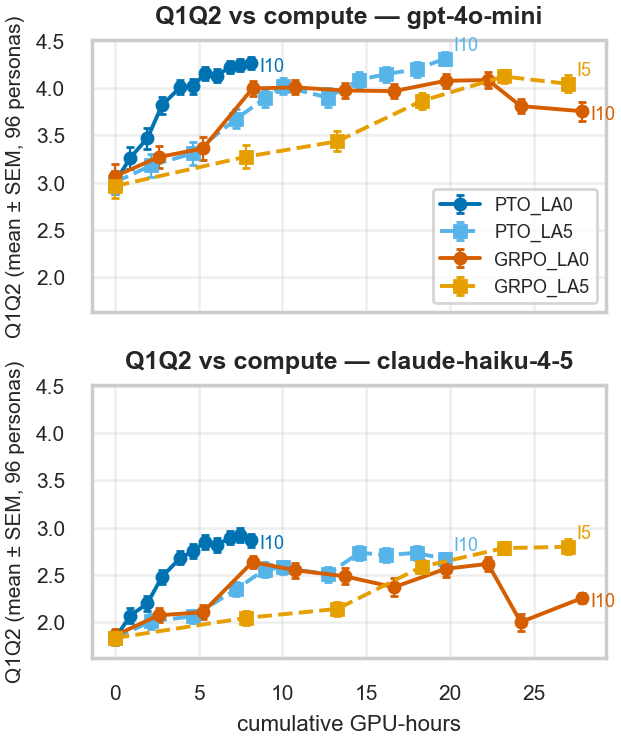
\includegraphics[width=\linewidth]{figures/compute_axis_fig_trajectory_col.png}
  \caption{\QQ{} (mean $\pm$ SE over 96 personas) against cumulative GPU-hours, training oracle
    (top) and held-out judge (bottom); last points labelled with their iteration (legend:
    LA0 $=$ \Kz{}, LA5 $=$ \Kf{}). GRPO \Kf{} ends at iteration~5 and $27.1$\,\gpuh{}, the spend of
    GRPO \Kz{}'s ten.}
  \label{fig:trajectory}
\end{figure}

\begin{table}[t]
  \centering\footnotesize
  \setlength{\tabcolsep}{3pt}
  \begin{tabular}{@{}l rr rr@{}}
    \toprule
    & \multicolumn{2}{c}{PTO} & \multicolumn{2}{c}{GRPO} \\
    \cmidrule(lr){2-3}\cmidrule(lr){4-5}
    & \Kz{} & \Kf{} & \Kz{} & \Kf{} \\
    \midrule
    generate (h)      & $1.32$ & $1.37$ & $1.21$ & $0.42$ \\
    build (h)         & $5.67$ & $16.80$ & --- & --- \\
    train (h)         & $1.13$ & $1.51$ & $26.69$ & $26.66$ \\
    total (\gpuh{})   & $8.12$ & $19.68$ & $27.91$ & $27.08$ \\
    per iteration (h) & $0.81$ & $1.97$ & $2.79$ & $5.42$ \\
    median step (s)   & $6.8$ & $6.9$ & $78.9$ & $155.8$ \\
    \midrule
    \multicolumn{5}{@{}l}{\emph{\Kf{}/\Kz{} ratio}} \\
    per iteration          & \multicolumn{2}{c}{$2.42$} & \multicolumn{2}{c}{$1.94$} \\
    per step, it.\ 3--5    & \multicolumn{2}{c}{$1.02$--$1.04$} & \multicolumn{2}{c}{$1.91$--$1.97$} \\
    API calls, it.\ 1--5   & \multicolumn{2}{c}{$2.08$} & \multicolumn{2}{c}{$2.25$} \\
    \bottomrule
  \end{tabular}
  \caption{What look-ahead costs (PTO arms and GRPO \Kz{}: ten iterations; GRPO \Kf{}: five).
    GPU-hours reconstructed from artifact times (\S\ref{sec:setup}); PTO pays for look-ahead in
    the preference-tree build, GRPO inside the optimizer step. API
    calls $=$ training-time oracle $+$ patient-simulator calls over iterations 1--5:
    $145{,}291/69{,}941$ (PTO), $338{,}476/150{,}427$ (GRPO); Table~\ref{tab:api}.}
  \label{tab:cost}
\end{table}

\paragraph{Look-ahead roughly doubles the price of a step.} Once GRPO \Kf{}'s look-ahead
batching had settled (iterations 3--5; Appendix~\ref{app:repro}) its median optimizer step took
$155.6$/$155.8$/$150.2$\,s against \Kz{}'s $79.2$/$79.4$/$78.6$\,s: ratios
$1.965$/$1.962$/$1.911$ (Table~\ref{tab:cost}). Per iteration GRPO \Kf{} costs
$5.416/2.791 = 1.94\times$ \Kz{}, so its five iterations ($27.08$\,\gpuh{}) match \Kz{}'s ten
($27.91$; Figure~\ref{fig:trajectory}). PTO pays in the build phase, where the ratio is
$16.80/5.67 = 2.96\times$ and the whole iteration $1.968/0.812 = 2.42\times$.

\paragraph{The API multiplier is the patient, not the oracle.} Oracle calls per candidate are
matched by construction: over iterations 1--5 the \Kf{}/\Kz{} call ratio is
$59{,}177/59{,}991 = 0.99$ for PTO and $141{,}237/143{,}548 = 0.98$ for GRPO (the oracle only
reads longer transcripts, $1.2$--$1.4\times$ the characters; Table~\ref{tab:api}). Each \Kf{} candidate adds $2.6$--$2.9$
patient-simulator calls in its tail, so patient calls rise $8.7\times$ (PTO) and $28.7\times$
(GRPO), and total API calls $2.08\times$ / $2.25\times$.

\paragraph{At matched budget, \Kf{} never significantly beats \Kz{} on the training oracle.}
The budget sweep (Table~\ref{tab:app:sweepK}, Figure~\ref{fig:sweep}) compares, at each of the
\Kf{} arm's cumulative budgets, the best checkpoint each arm reached for that money (selected on
the grader's \QQ{}, persona-paired). Signs in this and the next paragraph are $K{=}5$
minus $K{=}0$. Under the training oracle PTO \Kf{} is behind at every intermediate budget,
Holm-significantly through $14.6$\,h --- $-0.700$ at $4.6$\,h (\dz{} $-0.81$; its iteration~2
against \Kz{}'s iteration~4), $-0.174$ at $14.6$\,h (\dz{} $-0.35$, $p_{\text{Holm}}{=}.012$)
--- n.s.\ at $16.2$ and $18.0$\,h ($-0.116$, $-0.063$), and edges ahead only at the top,
$+0.047$ at $19.7$\,h (\dz{} $0.10$, CI $[-0.054, 0.142]$; iteration~10 vs~10). GRPO \Kf{} is
behind through $18.3$\,h --- $-0.088$ at $7.8$\,h (n.s.), $-0.569$ at $13.3$\,h (\dz{} $-0.74$),
$-0.143$ at $18.3$\,h (\dz{} $-0.28$, $p_{\text{Holm}}{=}.040$) --- and draws level from
$23.2$\,h on: $+0.038$ (\dz{} $0.07$, CI $[-0.053, 0.137]$; iteration~4 vs \Kz{}'s~8, the same
pair at $27.1$\,h because iteration~5 does not improve on~4 under the oracle). We quote the sweep
as a curve, not a row, because the lever's sign is a function of budget.

\paragraph{Under the held-out judge the two methods part.} GRPO \Kf{} ends ahead: $+0.147$ at
$23.2$\,h (\dz{} $0.33$, $p_{\text{Holm}}{=}.012$) and $+0.161$ at $27.1$\,h (\dz{} $0.31$, CI
$[0.057, 0.263]$, $p_{\text{Holm}}{=}.020$; iteration~5 vs \Kz{}'s~3). PTO \Kf{} stays behind:
$-0.186$ at $19.7$\,h (\dz{} $-0.32$, CI $[-0.301, -0.072]$, $p_{\text{Holm}}{=}.011$;
iteration~7 vs~9). Selecting and scoring on the same grader flatters it; crossing the two
(Appendix~\ref{app:tables}) keeps GRPO \Kf{}'s lead in one direction ($+0.166$, \dz{} $0.27$,
$p_{\text{Holm}}{=}.035$) but not the other ($+0.048$, n.s.), and keeps PTO \Kf{} behind
whenever the held-out judge selects or scores ($-0.153$, \dz{} $-0.27$,
$p_{\text{Holm}}{=}.023$ with the judge selecting and the oracle scoring; $-0.199$, \dz{}
$-0.31$, $p_{\text{Holm}}{=}.065$ the other way round) --- only the same-oracle combination
yields the $+0.047$ above.

\paragraph{PTO beats GRPO at matched budget under both graders and both $K$.} At \Kz{} and PTO's
top budget of $8.1$\,\gpuh{}, PTO's best checkpoint leads GRPO's by $+0.900$ (\dz{} $1.09$)
under the training oracle and $+0.814$ (\dz{} $1.39$) under the held-out judge,
$p_{\text{Holm}}{<}.001$ in every select/score combination; at \Kf{} and $19.7$\,\gpuh{} by
$+0.445$ (\dz{} $0.67$) and $+0.149$ (\dz{} $0.29$,
$p_{\text{Holm}}{=}.007$; Table~\ref{tab:app:sweepMethod}), though the \Kf{} held-out lead thins
to $+0.081$ (\dz{} $0.13$, n.s.) when the oracle selects and the judge scores
(Appendix~\ref{app:tables}). The optimizer gap is far larger than anything the $K$ lever moves
at any budget.
